\chapter{Additional R Diagnostic and E3 Image Archive}
\label{app:e3_archive}

\section{Additional R Executions and Source Precision}
Tables~\ref{tab:e1_rstar_all} and~\ref{tab:e1_rstar_ids} report the five additional outcomes and original identifiers.
\begin{table}[tbp]\centering\footnotesize
\caption[Additional R diagnostic runs]{All five \(R^{*}\) executions on 19 October, calculated from unrounded source CSVs and displayed to three decimals. The first diagnostic precedes four extension runs. These do not replace the original R1--R5. Time is first automatic procedure completion; pass speed uses the successful loaded-pass support.}
\label{tab:e1_rstar_all}\begin{tabular}{lrrrr}
\toprule
Run & Time (s) & $J_{\mathrm{excess}}$ (N\,s) & Peak (N) & Pass (mm/s) \\
\midrule
R$^{*}$1 & 22.481 & 0.000 & 21.488 & 10.696 \\
R$^{*}$2 & 25.319 & 0.000 & 22.000 & 10.887 \\
R$^{*}$3 & 25.520 & 0.000 & 20.541 & 10.886 \\
R$^{*}$4 & 25.458 & 0.000 & 22.727 & 10.822 \\
R$^{*}$5 & 25.420 & 0.000 & 20.944 & 10.915 \\
\bottomrule
\end{tabular}

\end{table}

The original per-run precision CSV and 17-page additional-R report describe the same five executions. Their identities, session/configuration identifiers, and template hashes are verified against the stored run contexts and input manifest. The first run uses configuration \path{e1ct_6c29a198a24df7a2}; repeats 2--5 use \path{e1ct_c5c424abc45fac4c}. All share the frozen template with SHA-256 prefix \texttt{1616a9f1bbb68df6}, the recorded feed, +18 N target, and v2 evaluator/observer. These identifiers preserve the one-then-four collection history.

\begin{table}[tbp]\centering\small
\caption[Original additional-R run identifiers]{Original identifiers for the additional \(R^{*}\) cohort. Full configuration and input hashes are supplied in the results manifest.}
\label{tab:e1_rstar_ids}\begin{tabular}{ll}
\toprule
Run & Original run identifier \\
\midrule
R$^{*}$1 & \texttt{E1\_CT\_NOMINAL\_R\_r1\_20261019T140517\_0921f1508b} \\
R$^{*}$2 & \texttt{E1\_CT\_NOMINAL\_R\_r2\_20261019T141109\_d8d222935d} \\
R$^{*}$3 & \texttt{E1\_CT\_NOMINAL\_R\_r3\_20261019T141211\_32499d64f6} \\
R$^{*}$4 & \texttt{E1\_CT\_NOMINAL\_R\_r4\_20261019T141312\_586a744e36} \\
R$^{*}$5 & \texttt{E1\_CT\_NOMINAL\_R\_r5\_20261019T141415\_bc2827864a} \\
\bottomrule
\end{tabular}

\end{table}

Reaggregation of the unrounded times gives \RstarTimeMeanPrecision~s and sample SD \RstarTimeSDPrecision~s, reproducing the displayed \EoneRstarTime\(\pm\)\EoneRstarTimeSD~s. The source-derived values and original identifiers are retained in \path{data/e1_rstar_source_runs.csv}. All five zero excess integrals and the shorter first run remain included.

\section{E3 Main-Run Pixel Areas}
Table~\ref{tab:e3_all_runs} lists the native-pixel areas for every main selected run.
\begin{table}[tbp]\centering\footnotesize
\caption[Individual E3 main-run image areas]{All 20 main selected N/P1/D1/D2 runs. Native-pixel areas are reproduced from the original RGB and frozen annotations and agree with the stored masks, CSVs, and image report. Percentages use Equation~\eqref{eq:e3_removal}. D1-4's final area and percentage remain null. Image evaluability is not procedure success.}
\label{tab:e3_all_runs}\begin{tabular}{lrrrl}
\toprule
Run & $A_{\mathrm{before}}$ (px) & $A_{\mathrm{after}}$ (px) & Removal (\%) & Note \\
\midrule
N-1 & 837 & 0 & 100.000 & image evaluable \\
N-2 & 879 & 0 & 100.000 & image evaluable \\
N-3 & 699 & 0 & 100.000 & image evaluable \\
N-4 & 697 & 0 & 100.000 & image evaluable \\
N-5 & 712 & 0 & 100.000 & image evaluable \\
P1-1 & 858 & 31 & 96.387 & image evaluable \\
P1-2 & 846 & 6 & 99.291 & image evaluable \\
P1-3 & 772 & 11 & 98.575 & image evaluable \\
P1-4 & 846 & 2 & 99.764 & image evaluable \\
P1-5 & 799 & 50 & 93.742 & image evaluable \\
D1-1 & 546 & 41 & 92.491 & image evaluable \\
D1-2 & 676 & 0 & 100.000 & image evaluable \\
D1-3 & 680 & 0 & 100.000 & image evaluable \\
D1-4 & 700 & \NA & \NA & tool occlusion \\
D1-5 & 798 & 0 & 100.000 & image evaluable \\
D2-1 & 768 & 79 & 89.714 & image evaluable \\
D2-2 & 738 & 13 & 98.238 & image evaluable \\
D2-3 & 794 & 128 & 83.879 & image evaluable \\
D2-4 & 743 & 13 & 98.250 & image evaluable \\
D2-5 & 684 & 12 & 98.246 & image evaluable \\
\bottomrule
\end{tabular}

\end{table}

The source-derived per-run identities and areas are captured in \path{data/e3_source_area_runs.csv}. Their ratios reproduce the reported main condition means and sample SDs. P1 ranges from 93.742 to 99.764\%, evaluable D1 from 92.491 to 100.000\%, and D2 from 83.879 to 98.250\%. The eight 100\% observations (five N and D1-2/3/5) mean black-ink nondetection under the established criterion. Figure~\ref{fig:e3_lowest_removal} preserves D2-3, the lowest observed individual removal, including all 128 residual pixels.

\begin{figure}[tbp]\centering
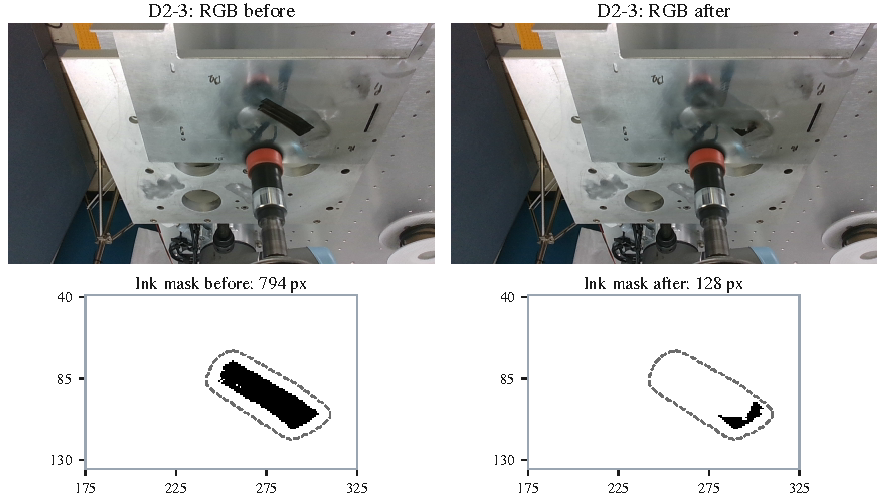
\includegraphics[width=\linewidth]{figures/e3_D2-3_native_evidence.pdf}
\caption[Lowest observed E3 removal, D2-3]{D2-3: original RGB and unchanged masks. The 794 initial and 128 residual pixels give 83.879\% removal. The common native-coordinate crop, dashed ROI, and black ink pixels follow the main evidence figures. This observed value is retained in D2's five-run mean.}
\label{fig:e3_lowest_removal}
\end{figure}

\section{Occlusion, Interruption, and P2 Exclusion}
Table~\ref{tab:e3_p2_archive} preserves the five excluded P2 image records. Figures~\ref{fig:e3_d1_occlusion} and~\ref{fig:e3_p2_occlusion} show the retained interruption and occlusion evidence.
\begin{table}[tbp]\centering\footnotesize
\caption[Executed P2 archive records]{P2 was executed five times and remains in the original 25-run selection. Every final photograph is tool-occluded. The initial areas are retained; whole-stain final areas and removal percentages are unavailable, not zero. P2 is outside the main four-condition removal evaluation.}
\label{tab:e3_p2_archive}\begin{tabular}{lrrl}
\toprule
Run & $A_{\mathrm{before}}$ (px) & Image result & Original stop \\
\midrule
P2-1 & 777 & unavailable & \texttt{operator\_finish} \\
P2-2 & 773 & unavailable & \texttt{operator\_finish} \\
P2-3 & 652 & unavailable & \texttt{operator\_finish} \\
P2-4 & 717 & unavailable & \texttt{operator\_finish} \\
P2-5 & 778 & unavailable & \texttt{operator\_finish} \\
\bottomrule
\end{tabular}

\end{table}

D1-4 retains \texttt{manual\_abort}; its interruption-time diagnostic frame contains visible residual marking and final tool occlusion. The report identifies the frame as received 34.5 ms before the abort request (source stamp approximately 0.55 s before it). No post-HOME photograph is available. The visible region is not used to estimate hidden total residual area. P2's initial frames are same-run pre-execution raw RGB, replacing initially occluded photographs; the final occlusion remains. These records are not removed or renamed in the archive.

\begin{figure}[tbp]\centering
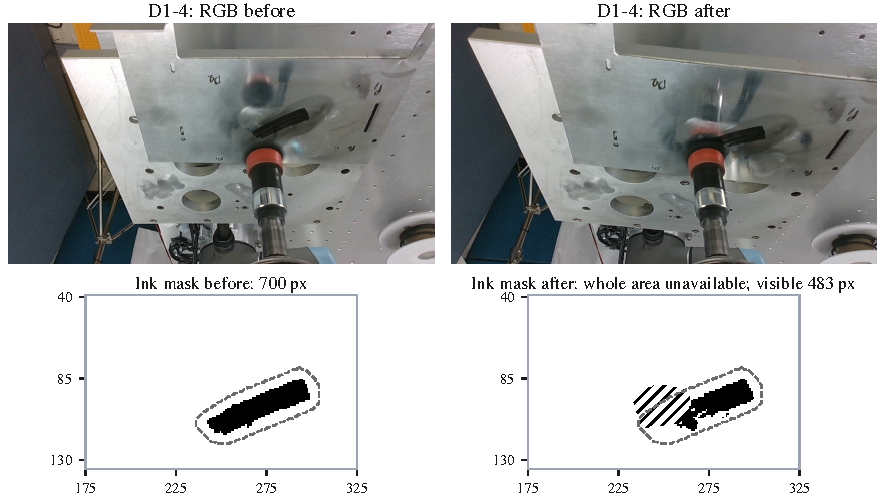
\includegraphics[width=\linewidth]{figures/e3_D1-4_native_evidence.pdf}
\caption[D1-4 retained interruption and occlusion evidence]{D1-4 original pre-task RGB and interruption-time diagnostic frame, with the unchanged saved masks. Hatching denotes final tool occlusion in the initial-frame reference grid. Visible residual ink is retained; hidden residual area is not estimated and whole-stain removal remains null. The existing surface-feature alignment is used for the occlusion display only.}
\label{fig:e3_d1_occlusion}
\end{figure}

\begin{figure}[tbp]\centering
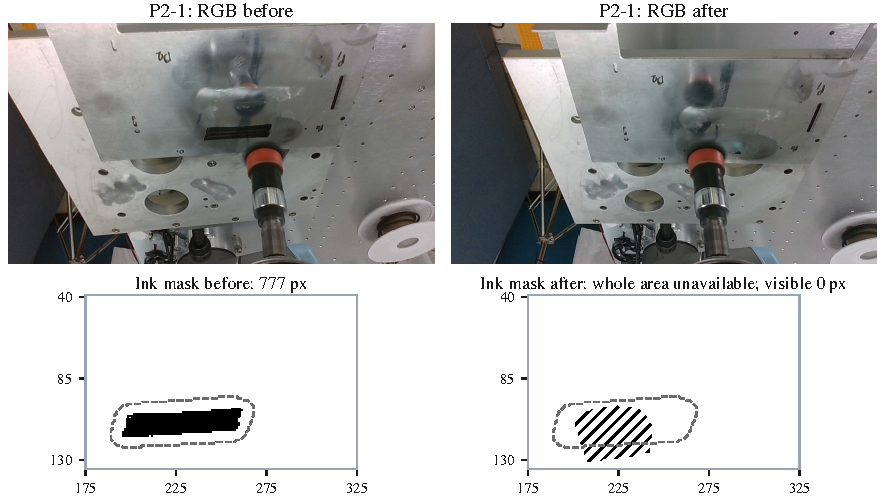
\includegraphics[width=\linewidth]{figures/e3_P2-1_native_evidence.pdf}
\caption[P2 retained final occlusion example]{P2-1 original pre-execution initial RGB and final image, with saved masks and occlusion hatching. The same-run initial replacement exposes the marking; final tool occlusion prevents whole-stain measurement. The mask display uses the established surface homography without reconstructing hidden image content. All five P2 records remain in the 25-run archive.}
\label{fig:e3_p2_occlusion}
\end{figure}

\section{Reused Segmentation Sensitivity and Procedure Diagnostics}
The report's sensitivity check keeps annotations and ROI fixed and changes the gray threshold equally in before/after images. Table~\ref{tab:e3_sensitivity} reproduces the published condition means at their printed precision; no new threshold or manual boundary is selected.

\begin{table}[tbp]\centering\small
\caption[Archived E3 threshold sensitivity]{Existing sensitivity results from the image report, p.36. Values are condition-mean percentages; main gray threshold is 45. These are not sample SD or confidence intervals. D1 uses four images throughout.}
\label{tab:e3_sensitivity}
\begin{tabular}{lrrr}\toprule
Condition & gray \(\leq40\) & gray \(\leq45\) & gray \(\leq50\) \\ \midrule
N & 100.000 & 100.000 & 100.000 \\
P1 & 97.912 & 97.552 & 96.914 \\
D1 & 98.124 & 98.123 & 98.056 \\
D2 & 94.659 & 93.665 & 92.932 \\
\bottomrule\end{tabular}
\end{table}

The archived v2 procedure outcomes are 8 completed and 17 \texttt{observation\_unavailable} in the original 25-run selection, with 24/25 HOME returns. The 25-page execution report, its per-run metrics CSV, and the selected run contexts retain these same identities and diagnostic labels. They are auxiliary procedure records on that archive, not removal successes or outcomes for the main 20-run subset. Image inclusion is independent of them; the force/path evaluator is not rerun for the image analysis.

\section{Evidence Availability and Reproduction}
The 39-page image report's pp.10--34 contain one RGB/ROI/mask evidence panel per selected run. The original \path{image_pair_manifest.json} and CSV, \path{analysis_config.json}, \path{annotations.json}, and \path{occluded_runs.csv} are linked to the frozen 25-run selection. All 50 original RGB files match the recorded file hashes. The saved per-run contexts confirm the registered offsets, common C checkpoint/normalizer identifiers, and condition-specific termination implementations.

Reprocessing the original RGB with the unchanged algorithm, inclusive gray threshold 45, and saved polygon/ROI settings reproduces all 25 initial areas, 19 available final areas, and visible-residual diagnostics for the six occluded cases. The 25 initial ink masks, 25 final aligned masks, and 25 initial ROI arrays are pixel-identical to their archived counterparts. All 19 evaluable pairs use verified identity surface registration. The six occluded pairs retain their original surface-feature alignment and unavailable whole-stain values. This is RGB-level computational reproduction, in addition to CSV aggregation and mask comparison; it is not an independent reassessment of the manual semantic labels.

The native figure assets preserve the original \(424\times240\) photographs. Binary-mask panels use the same \(x=175{:}325\), \(y=39{:}135\) crop and scale before/after and across displayed cases. Nearest-neighbor display preserves individual pixels; dashed vector ROI boundaries and occlusion hatching are annotations. No enhanced or generated photograph is used for measurement. The supplied display manifest records the selected original run IDs and hashes. Full source mapping, verification levels, software versions, and commands are supplied separately from the standalone document build.
